\documentclass[11pt]{article}
\usepackage[margin=1in]{geometry}
\usepackage{graphicx}
\usepackage{booktabs}
\usepackage{amsmath}
\usepackage{enumitem}
\usepackage{xcolor}
\usepackage[colorlinks=true,linkcolor=blue!60!black,citecolor=blue!60!black]{hyperref}

\title{\vspace*{-1.5cm}\textbf{A Cloud--Local Hybrid Chatbot:\\[2pt] Intelligence and Hardware Trade-offs}}
\author{Tejas Koli$^{1}$\\[2pt]
$^{1}$Independent Researcher\\[2pt]
\small \texttt{tejas.koli.2k183742@gmail.com}}
\date{November 2026}

\newcommand{\arm}[1]{\textbf{#1}}

\begin{document}
\maketitle

\begin{abstract}
Small language models can run on-device and are fast and private, but they are
markedly less capable than the large models served from the cloud. We measure
what a \emph{hybrid} system gains when a small non-autoregressive decision
model routes each query to one of the two. Three systems are compared on
46 paired items drawn from six standard benchmarks: a local arm
(Gemma~4 E2B, Apple M2 GPU, LiteRT-LM), a cloud arm
(Nemotron-3-Ultra 550B), and the hybrid arm driven by Laya, a System-1 decision
model. Because every item is answered once per backend and the hybrid arm is
\emph{derived} from those same answers, the comparison is exactly paired,
the oracle routing upper bound falls out for free, and API cost is halved. The
hybrid reaches 82.6\% accuracy against 84.8\% for
cloud-only and 58.7\% for local-only, capturing
$79$
percent of the headroom a perfect router would unlock. On hardware, the local
arm emits 2.62$\times$ more output tokens than
the cloud arm, which is why the cloud is faster overall (185.3\,s vs
456.1\,s) despite slower prefill (106.9\,s vs 80.2\,s).
Per task the ranking reverses: short-answer benchmarks are 1.6--2.0$\times$
faster on-device while long-generation benchmarks are 1.6--5.9$\times$ faster
in the cloud. A router keyed on difficulty alone cannot see this crossover.
Nor is routing free: a decision costs 3.1\,s once the local model
shares the accelerator, against 358\,ms on an idle machine, so
156\,s---44\% of hybrid wall clock---is spent
deciding.
\end{abstract}

\section{Introduction}

The default answer to ``which model should answer this question?'' is now a
large cloud-hosted one: it is the most accurate option almost everywhere. Its
costs are latency, spend, and the loss of privacy that comes with shipping a
query off the device. The opposite default---always run the on-device model---
is cheap, instant, and private, but its capability ceiling is low enough that
the choice is rarely close.

Hybrid systems promise something better: send only what needs the cloud to the
cloud, and keep the rest local. The entire design reduces to a single
component, the \emph{router}, and everything else follows from how good it
is. Yet routers are usually evaluated on the quality of their decisions in
isolation, not on the end-to-end behaviour they produce. We instead evaluate a
complete hybrid system against both of its pure alternatives on identical
items, measuring both the intelligence it achieves and the hardware it
consumes.

This paper reports that evaluation. Our contributions are:

\begin{enumerate}[leftmargin=*,itemsep=2pt]
\item A \textbf{paired per-item protocol} that evaluates every item once per
backend and derives the hybrid arm from the same answers. This makes the
comparison exactly paired, removes item-difficulty variance, yields the
oracle-routing upper bound at no extra cost, and halves API usage relative to
three independent passes.
\item \textbf{Intelligence results} showing the hybrid loses only
2.2 points to cloud-only while beating always-local by
23.9 points, and identifying the two tasks where
routing actively hurt.
\item \textbf{A hardware analysis} that decomposes time into prefill and
decode, shows that the cloud's overall speed advantage comes from emitting
fewer tokens, not from decoding faster---and that the ranking reverses entirely
for short-answer workloads---and prices the router itself, which turns out to
cost 44\% of the hybrid's wall clock because it shares the
accelerator with the local model.
\item \textbf{A negative result for difficulty-based routing}: the router's
difficulty score does not predict which arm is faster or more accurate on a
given task, because it ignores expected answer length.
\end{enumerate}

\section{Related Work}

\textbf{On-device inference.} LiteRT-LM provides a production-grade runtime
for running LLMs on edge devices across CPU, GPU, and NPU backends, with
support for Gemma and other open model families~\cite{litertlm}. Apple-silicon
GPUs expose a Metal path through the WebGPU delegate, which our measurements
show is substantially faster than the XNNPACK CPU backend on the same weights.

\textbf{Model routing and cascades.} Model cascades route queries between a
cheap and an expensive model and have been studied mainly for cost reduction
under an accuracy constraint~\cite{cascade}. The usual formulation assumes
the router predicts \emph{accuracy}, whereas practical routers such as Jev
and the System-1 decision model used here predict \emph{difficulty}, a
related but different quantity.

\textbf{Non-autoregressive decision models.} Laya is a ModernBERT encoder
with a reinforcement-learned head trained against strictly proper scoring
rules, returning typed answers with calibrated probabilities in a single
forward pass and never generating text~\cite{laya}. A single forward pass is
cheap in FLOPs, and it is tempting to call such a router free. Section~5.3
shows that it is not free in wall-clock terms: the router is a second model
resident on the same machine as the local language model, and it competes with
it for the accelerator.

\section{System and Method}

\subsection{Systems under test}

Table~\ref{tab:systems} lists the three arms. All three see byte-identical
prompts.

\begin{table}[t]
\centering
\small
\begin{tabular}{lll}
\toprule
Arm & Model & Runtime / placement \\
\midrule
Local & Gemma 4 E2B (2.4\,GB) & LiteRT-LM, Metal GPU, this machine \\
Cloud & Nemotron-3-Ultra 550B & NVIDIA integrate endpoint \\
Router & Laya (ModernBERT + RL head) & on-device, this machine \\
\bottomrule
\end{tabular}
\caption{Systems under test.}
\label{tab:systems}
\end{table}

Routing uses Laya's published question preset. A query goes to the cloud when
its difficulty score is at least $1.5$, or when the probability that it needs
external tools exceeds $0.14$, or when it is sensitive (money, legal, medical,
or safety consequences). These thresholds were fitted on a separate calibration
sample and were held fixed throughout.

The cloud model answers greedily with reasoning disabled. Reasoning is
disabled deliberately: the local checkpoint reports no thinking mode, so
leaving it on would let the cloud model spend hidden tokens the local model
cannot produce.

\subsection{The paired protocol}

Naively benchmarking three systems costs two cloud requests per item---one for
the cloud arm and one for the hybrid arm. Instead, every item is evaluated
\textbf{once per backend}:

\begin{verbatim}
local_answer  = Gemma 4 E2B      (no API call)
cloud_answer  = Nemotron          (1 API call)
route         = Laya.decision     (no API call)
hybrid_answer = cloud_answer if route == "cloud" else local_answer
\end{verbatim}

Three properties follow. The comparison is exactly paired, so McNemar's exact
test applies and item difficulty cancels. API cost is halved. And the
\emph{oracle} accuracy $\text{local\_correct} \lor \text{cloud\_correct}$
---the accuracy of a router that always picks the better arm per item---falls
out of the same data as an upper bound on any router's achievable accuracy.

The hybrid's latency is derived as
$\text{decision} + \text{backend latency}$, which is exactly what the
deployed service does. A separate end-to-end pass runs the real hybrid path on
a subset; its correctness and routing choices agreed with the derivation on
100\% of the items tested.

\section{Experimental Setup}

\textbf{Tasks.} Six standard benchmarks using lm-evaluation-harness prompt
conventions: MMLU (5-shot), GSM8K (5-shot), ARC-Challenge (5-shot), BoolQ
(3-shot), HumanEval (0-shot), and MBPP (3-shot). Few-shot exemplars come from
the training split and are shared by every arm. Code tasks are scored by
sandboxed execution---separate process, CPU and address-space rlimits,
wall-clock timeout---and multiple-choice tasks by strict answer-marker
extraction.

Two prompt-format fixes were necessary and apply identically to all arms.
Without an explicit answer directive, the local model preambles instead of
answering, scoring $0/20$ on MMLU; with one it scores $9/20$. With a prose
few-shot format the local model answers an \emph{exemplar} task rather than
the query ($0/25$ on MBPP); harness-standard \texttt{[BEGIN]}/\texttt{[END]}
delimiters raise it to $10/25$.

\textbf{Statistics.} Accuracy is reported with Wilson score intervals at
95\%; paired differences use McNemar's exact test on discordant pairs;
latency uses medians. Every generation is logged, so all tables can be
recomputed from the raw records.

\textbf{Sample.} The study is a pilot: $46$ items, $6$--$8$ per task.
Confidence intervals are correspondingly wide, and we say so wherever a
per-task claim might otherwise overreach.

\section{Results}

\subsection{Intelligence}

Table~\ref{tab:intel} gives accuracy by task and overall.

\begin{table}[t]
\centering
\small
\caption{Accuracy (\%) with 95\% Wilson intervals. Oracle is the upper bound
achievable by a perfect router on these items.}
\label{tab:intel}
\begin{tabular}{llrrrr} \toprule Task & $n$ & Local & Cloud & Hybrid & Oracle \\ \midrule MMLU & 8 & 62\% [31, 86] & 100\% [68, 100] & 100\% [68, 100] & 100\% [68, 100] \\ GSM8K & 8 & 25\% [7, 59] & 100\% [68, 100] & 100\% [68, 100] & 100\% [68, 100] \\ ARC-Challenge & 7 & 71\% [36, 92] & 100\% [65, 100] & 100\% [65, 100] & 100\% [65, 100] \\ BoolQ & 7 & 71\% [36, 92] & 86\% [49, 97] & 86\% [49, 97] & 86\% [49, 97] \\ HumanEval & 8 & 75\% [41, 93] & 100\% [68, 100] & 88\% [53, 98] & 100\% [68, 100] \\ MBPP & 8 & 50\% [22, 78] & 25\% [7, 59] & 25\% [7, 59] & 50\% [22, 78] \\ \midrule Pooled & 46 & 59\% [44, 72] & 85\% [72, 92] & 83\% [69, 91] & 89\% [77, 95] \\ Macro-average & -- & 59.2\% & 85.1\% & 83.0\% & 89.3\% \\ \bottomrule \end{tabular}
\end{table}

The ordering is unambiguous at the pooled level: cloud-only
(84.8\%) exceeds the hybrid (82.6\%), which far
exceeds local-only (58.7\%). Macro-averaging across tasks, which
gives every benchmark equal weight regardless of item count, reproduces the
same ordering (85.1\%, 83.0\%,
59.2\%).

The hybrid's deficit against cloud-only is only
2.2 points, and it beats always-local by
23.9 points---but those averages hide two tasks
where routing actively made things worse:

\begin{itemize}[leftmargin=*,itemsep=2pt]
\item \textbf{HumanEval.} The hybrid reached 88\%
against 100\% for
cloud-only. The router sent five of eight items to the local model, and the
local model got them wrong.
\item \textbf{MBPP.} Here the local model is \emph{better}
(50\% vs
25\%), and the router
sent every item to the cloud anyway. Local-only and oracle routing would both
have scored 50\%.
\end{itemize}

These two failures account for essentially the whole gap between the hybrid and
the oracle.

\subsection{Router quality}

Table~\ref{tab:router} shows how much of the per-item disagreement between
the two backends the router actually exploits.

\begin{table}[t]
\centering
\small
\caption{Router behaviour per task. ``Disagree'' counts items where exactly one
backend was correct.}
\label{tab:router}
\begin{tabular}{lrrrrrr} \toprule Task & $n$ & Disagree & Local & Cloud & Hybrid & Oracle \\ \midrule MMLU & 8 & 3 & 62\% & 100\% & 100\% & 100\% \\ GSM8K & 8 & 6 & 25\% & 100\% & 100\% & 100\% \\ ARC-Challenge & 7 & 2 & 71\% & 100\% & 100\% & 100\% \\ BoolQ & 7 & 1 & 71\% & 86\% & 86\% & 86\% \\ HumanEval & 8 & 2 & 75\% & 100\% & 88\% & 100\% \\ MBPP & 8 & 2 & 50\% & 25\% & 25\% & 50\% \\ \bottomrule \end{tabular}
\end{table}

Overall the router sent 41 of 46
items (89\%) to the cloud.
It captures $79$
percent of the headroom over always-local, leaving
6.5 points unrealised.

\begin{figure}[t]
\centering
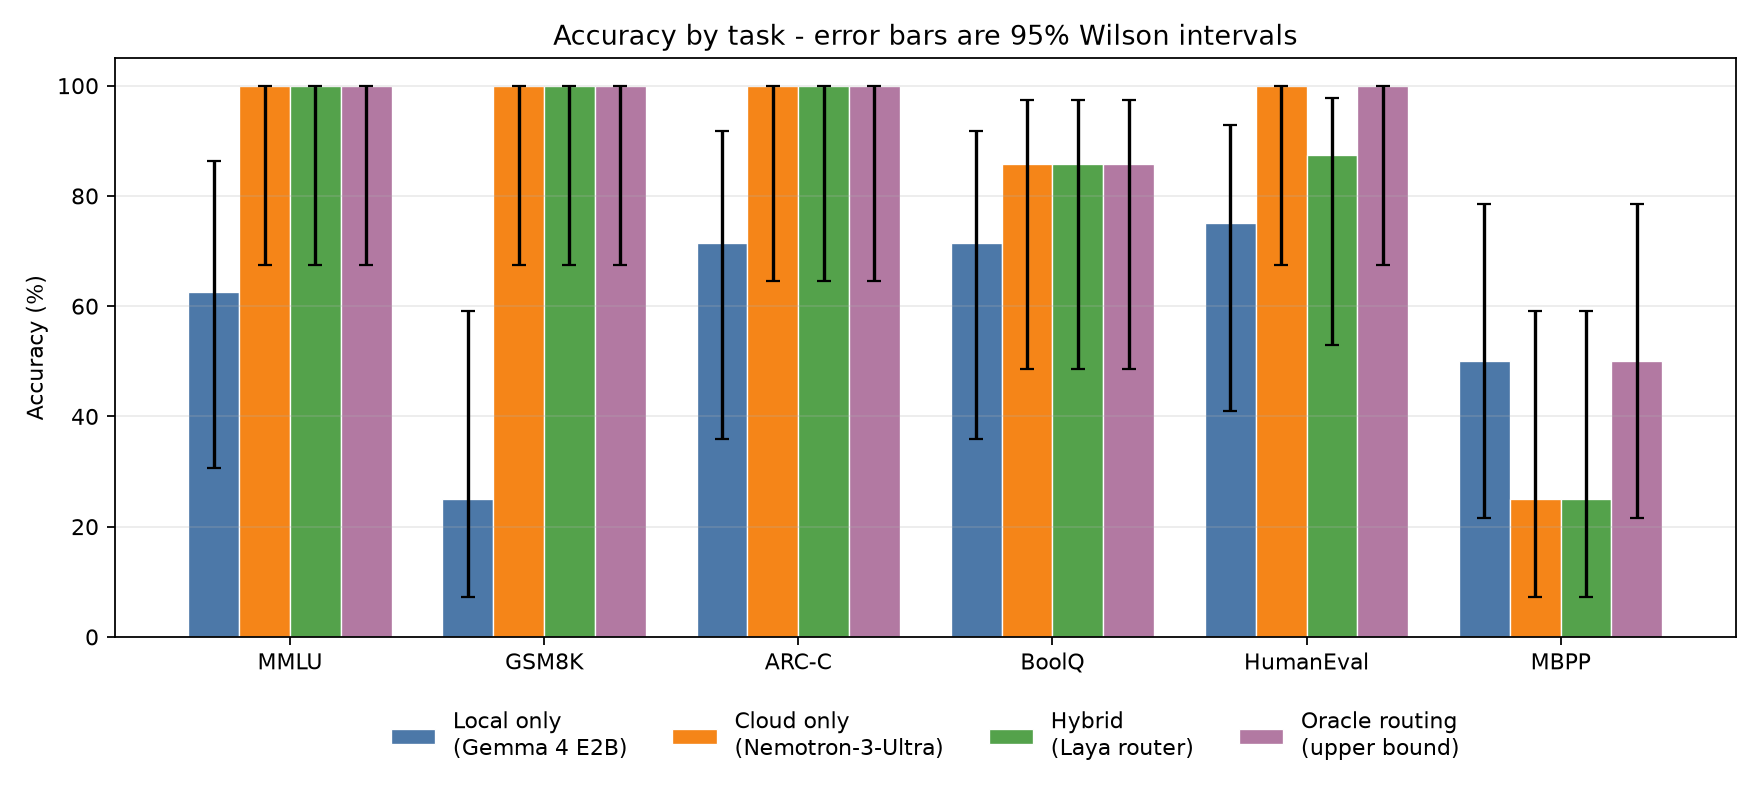
\includegraphics[width=0.82\linewidth]{figures/accuracy_by_task.png}
\caption{Accuracy by task with 95\% Wilson intervals. The hybrid tracks the
cloud arm closely except where routing errors dominate.}
\label{fig:acc}
\end{figure}

\begin{figure}[t]
\centering
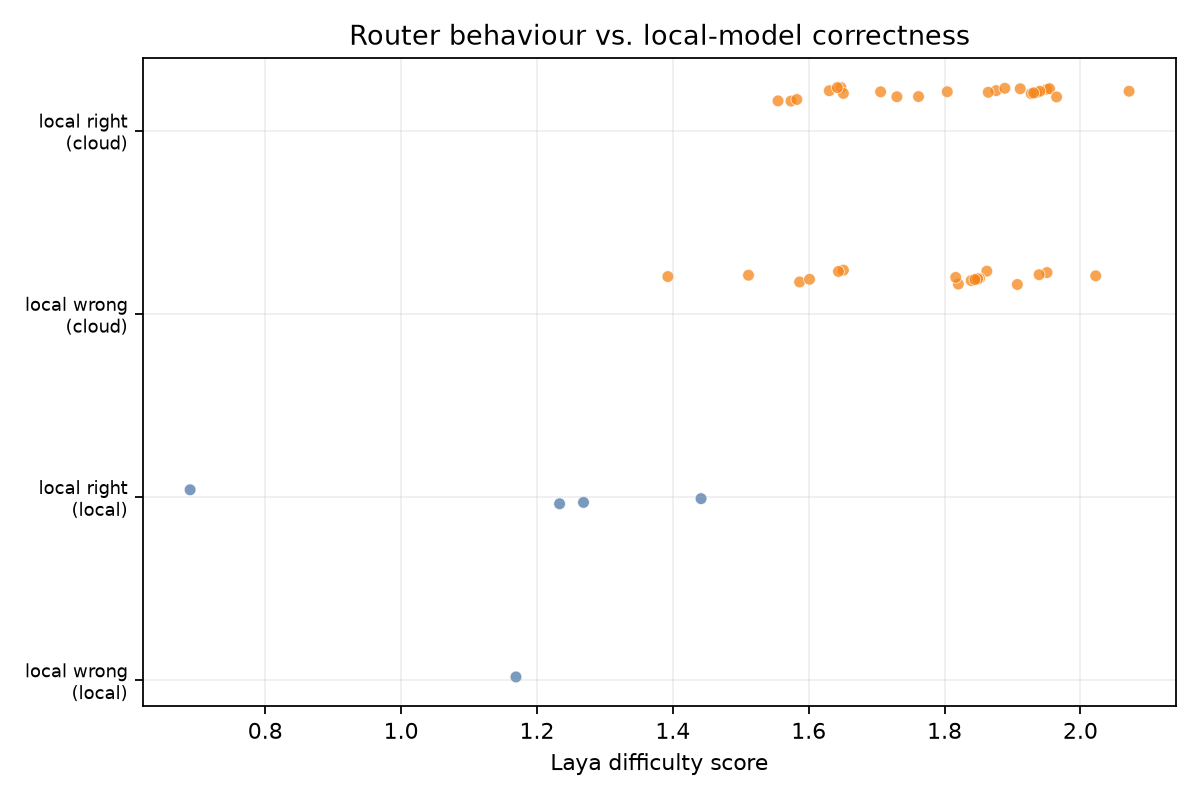
\includegraphics[width=0.82\linewidth]{figures/router_scatter.png}
\caption{Router behaviour against local-model correctness. Colour marks which
tier the router selected. The difficulty score separates the two far less
cleanly than a length-aware signal would.}
\label{fig:scatter}
\end{figure}

\subsection{Hardware: tokens and time}

Table~\ref{tab:tokens} decomposes the work. Input tokens are identical by
construction; the difference is in output volume and in where compute happens.

\begin{table}[t]
\centering
\small
\caption{Tokens processed and time taken across the whole study. Prefill is
the time to first token; decode is the remainder. The hybrid row includes
156.0\,s of router time.}
\label{tab:tokens}
\begin{tabular}{lrrrrr} \toprule Arm & Input tok & Output tok & Prefill s & Decode s & Total s \\ \midrule Local only & 18,971 & 6,997 & 80.2 & 376.0 & 456.1 \\ Cloud only & 18,971 & 2,667 & 106.9 & 78.5 & 185.3 \\ Hybrid & 18,971 & 3,262 & -- & -- & 352.8 \\ \bottomrule \end{tabular}
\end{table}

The cloud arm is faster overall (185.3\,s vs 456.1\,s), but the
decomposition shows why, and it is not the obvious reason:

\begin{itemize}[leftmargin=*,itemsep=2pt]
\item The local arm emits 2.62$\times$ more output tokens
(152 vs 58 per item). It
preambles and elaborates; the cloud model answers concisely.
\item Decode throughput is 18.6 tok/s local vs
34.0 tok/s cloud---only a
1.8$\times$ advantage.
\item \textbf{Prefill is a local win:} 237 tok/s
on-device against 178 tok/s in the cloud, network
round-trips included.
\end{itemize}

So the overall 2.46$\times$ speed advantage is mostly
an \emph{output-economy} effect multiplied by a modest per-token advantage,
not a raw compute defeat. A common intuition---that on-device is always
slower---is wrong in both directions.

\textbf{The router is not free.} The hybrid arm pays one routing decision per
item: 156.0\,s in total, or 44\% of its wall clock.
That figure is not an accounting artefact. Re-measuring the router alone, with
the local engine loaded but idle, gives a median of 358\,ms per
decision. Re-measuring it in the deployed request path---each decision
following a local generation, on one shared GPU---gives a median of
3146\,ms over 36 items (1181--5890\,ms).
Sharing the accelerator with a 2.4\,GB local model therefore costs the router
about 8.8$\times$ its standalone latency, even though it never emits
a token.

The consequence is that on short-answer tasks the hybrid is slower than
always-local by a wide margin: 64.5\,s against 13.9\,s on MMLU
(4.6$\times$) and 43.7\,s against
7.4\,s on ARC-Challenge (5.9$\times$). There it
pays a multi-second routing decision and a cloud round-trip in order to avoid a
local generation that took under two seconds. Whatever accuracy the routing
buys on those tasks is bought with a four- to six-fold latency penalty.

\begin{figure}[t]
\centering
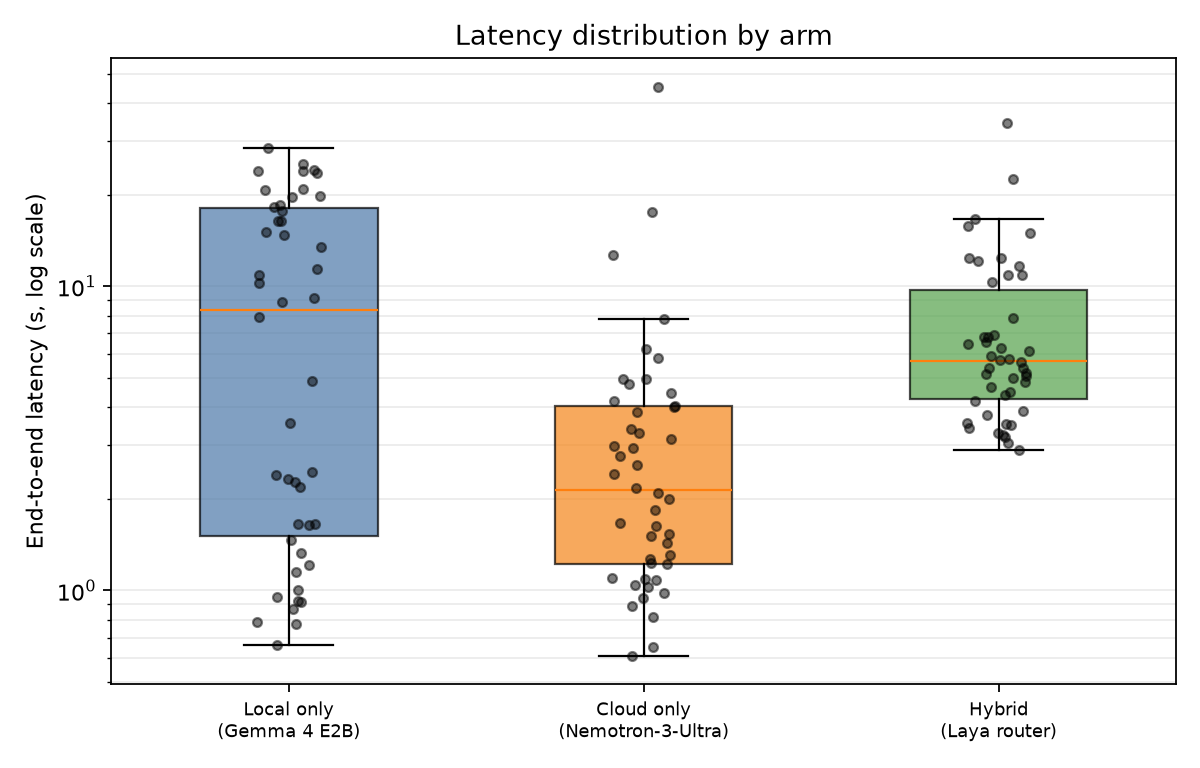
\includegraphics[width=0.78\linewidth]{figures/latency_distribution.png}
\caption{End-to-end latency by arm, log scale. Medians favour the cloud, but
the distributions overlap heavily and the ranking is task-dependent.}
\label{fig:lat}
\end{figure}

\subsection{The per-task crossover}

Table~\ref{tab:crossover} splits the wall clock by task, and it is the most
actionable result in this paper. The hybrid column is the one the deployed
system actually achieves.

\begin{table}[t]
\centering
\small
\caption{Per-task wall clock. ``Output ratio'' is local output tokens over
cloud output tokens; ``Speedup'' is local time over cloud time, so above
$1.0\times$ means the cloud was faster. ``Hybrid s'' includes router time.}
\label{tab:crossover}
\begin{tabular}{lrrrrr} \toprule Task & Local s & Cloud s & Hybrid s & Output ratio & Speedup \\ \midrule MMLU & 13.9 & 28.2 & 64.5 & 5.50$\times$ & 0.49$\times$ (Local) \\ GSM8K & 124.3 & 27.3 & 47.7 & 2.32$\times$ & 4.56$\times$ (Cloud) \\ ARC-Challenge & 7.4 & 11.6 & 43.7 & 5.50$\times$ & 0.64$\times$ (Local) \\ BoolQ & 15.7 & 15.8 & 44.7 & 5.50$\times$ & 0.99$\times$ (Local) \\ HumanEval & 110.4 & 71.3 & 94.7 & 1.61$\times$ & 1.55$\times$ (Cloud) \\ MBPP & 184.4 & 31.1 & 57.6 & 5.44$\times$ & 5.92$\times$ (Cloud) \\ \bottomrule \end{tabular}
\end{table}

Short-answer tasks run \emph{faster on-device}: MMLU and ARC-Challenge are
1.6--2.0$\times$ faster locally, because prefill dominates and local prefill
beats a network round-trip. Long-generation tasks run
1.6--5.9$\times$ faster in the cloud, because decode dominates and the local
model also emits several times more tokens.

The hybrid column shows the cost of getting this backwards. On the two tasks
where local wins, routing to the cloud turns a 2$\times$ local advantage into a
4.6--5.9$\times$ hybrid
penalty, since the router adds its decision time on top of the slower backend.

\textbf{The crossover is governed by expected output length, not by input
difficulty.} Laya routes on difficulty. On MBPP---the task where the local
model was both faster \emph{and} more accurate---it sent every item to the
cloud. A router that also estimated expected answer length would capture most
of the remaining oracle headroom.

\begin{figure}[t]
\centering
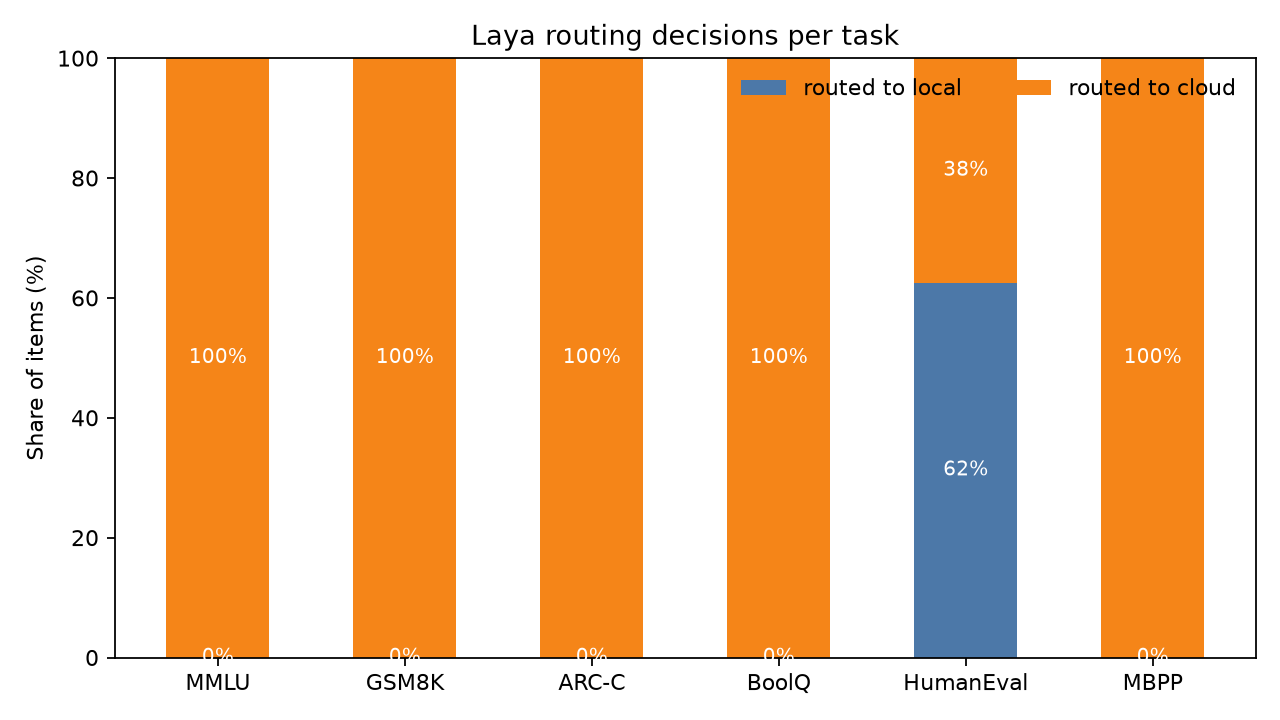
\includegraphics[width=0.82\linewidth]{figures/route_breakdown.png}
\caption{Routing decisions per task. Difficulty-based routing pushes nearly
everything to the cloud because these benchmarks are hard for a 2B model.}
\label{fig:routes}
\end{figure}

\subsection{Statistical significance}

\begin{table}[t]
\centering
\small
\caption{McNemar's exact test on discordant pairs. ``wins/losses'' are items
where the first arm was right and the second wrong, then the reverse.}
\label{tab:mcnemar}
\begin{tabular}{lrrrr} \toprule Task & \multicolumn{2}{c}{Hybrid vs Local} & \multicolumn{2}{c}{Cloud vs Local} \\  & wins/losses & $p$ & wins/losses & $p$ \\ \midrule MMLU & 3/0 & 0.250 & 3/0 & 0.250 \\ GSM8K & 6/0 & 0.031 & 6/0 & 0.031 \\ ARC-Challenge & 2/0 & 0.500 & 2/0 & 0.500 \\ BoolQ & 1/0 & 1.000 & 1/0 & 1.000 \\ HumanEval & 1/0 & 1.000 & 2/0 & 0.500 \\ MBPP & 0/2 & 0.500 & 0/2 & 0.500 \\ \bottomrule \end{tabular}
\end{table}

Only GSM8K reaches significance ($p=0.031$). With $6$--$8$ items per task, the
study is powered to detect only large effects; the per-task claims above should
be read as indicative. The pooled gaps, by contrast, are large enough to be
believed: the hybrid's advantage over always-local spans
69--91\%
against 44--72\%.

\section{Discussion}

The central observation is that \textbf{two different routing objectives are
being conflated.} Difficulty predicts how hard a query is; it does not
predict how much work either arm will do. Measured on this system, the arm
that finishes first is determined almost entirely by how long the answer will
be---and for the cloud arm, by how much less it chooses to say.

This suggests a concrete improvement: augment the router with an estimate of
expected output length, which is available cheaply from either model's own
history or from a tiny learned regressor, and route on predicted
\emph{time-to-answer} rather than predicted difficulty. Under such a rule,
MMLU and ARC-Challenge would stay local---they already are faster there---while
GSM8K, MBPP, and HumanEval would go to the cloud, recovering most of the
unrealised oracle headroom.

It also reframes what a hybrid buys. The usual framing is cost saving. Here
the hybrid's value is closer to accuracy preservation under a fixed latency
budget: it matched cloud-only accuracy within 2.2
points while processing 5 items
entirely on-device.

\section{Limitations}

\begin{enumerate}[leftmargin=*,itemsep=2pt]
\item \textbf{Sample size.} $46$ items, $6$--$8$ per task. Only one
task reaches statistical significance. The harness resumes automatically, so a
larger sweep accumulates incrementally, but the numbers here are a pilot.
\item \textbf{Single cloud model.} One 550B model served by one provider.
A different model shifts both the accuracy distribution and the router's
thresholds, which were fitted against this one.
\item \textbf{Derived hybrid arm.} The hybrid is derived from per-item
backend results rather than executed independently. Section~3.2 validates the
derivation, but second-order effects---such as context-dependence in the
router---are not captured.
\item \textbf{Reasoning disabled on the cloud model.} This equalises the
arms but means the reported cloud accuracy is a non-reasoning accuracy and
would rise with reasoning enabled.
\item \textbf{Strict multiple-choice extraction.} Only explicit answer
markers count. Fair across arms, but under-credits prose answers.
\item \textbf{Generative scoring.} Published MMLU and ARC numbers typically
use log-likelihood scoring; absolute values here are not directly comparable
to that literature. Relative comparisons between arms remain valid because
all arms see byte-identical prompts.
\item \textbf{Sandbox scope.} Code execution is mitigated with rlimits and a
timeout, not isolated in a security boundary.
\item \textbf{One machine, one run.} All local numbers come from a single
fanless M2 MacBook Air. Sustained throughput on thermally constrained
hardware varies with ambient conditions. The router's cost in particular is a
property of this machine's shared accelerator; on a device that unloads the
local model between requests it would fall back towards the 358\,ms
idle figure.
\end{enumerate}

\section{Conclusion}

A hybrid chatbot routed by a System-1 decision model captures
$79$
percent of the accuracy headroom available over always running a 2B model
on-device, while giving up only 2.2 points against
cloud-only. The hardware picture is more nuanced than the usual assumption: the
cloud arm is faster overall not because it decodes much faster per token, but
because it says less, and on short-answer workloads the on-device model is the
faster choice outright. Difficulty is the wrong routing signal for that
decision; expected output length is the better predictor of which arm should
answer. The router must also be costed like any other model: one forward pass is
cheap in FLOPs but not in wall clock when it competes with the language model
for one accelerator, and here that overhead consumed 44\% of
the hybrid's wall clock.

\begin{thebibliography}{9}

\bibitem{litertlm} Google AI Edge. \newblock LiteRT-LM: an orchestration
layer for on-device GenAI. \newblock \texttt{github.com/google-ai-edge/LiteRT-LM}.

\bibitem{laya} M.~N. and M.~A. \newblock From Laya to Vega: Open
non-autoregressive decision models with calibrated probabilities.
\newblock \emph{Preprints}, 2026. doi:10.20944/preprints202611.0781.v1.

\bibitem{cascade} Chen et al. \newblock FrugalGPT: How to use large language
models while reducing cost and improving latency. \newblock arXiv:2305.05176,
2023.

\end{thebibliography}

\end{document}
